\section{Motivating example: a parallel, pipelined graph computation}\label{s:lvars-motivation}

What applications motivate going beyond IVars and FIFO streams?
Consider applications in which independent subcomputations contribute
results to shared mutable data structures.  
Hindley-Milner type inference is one example: in a
parallel type-inference algorithm, each type variable monotonically
acquires information through unification.
Likewise, in control-flow analysis, the \emph{set} of
locations to which a variable refers monotonically \emph{shrinks}.  In
logic programming, a parallel implementation of conjunction might
asynchronously add information to a logic variable from different
threads.

To illustrate the issues that arise in computations of this nature,
consider a specific problem, drawn from the domain of \emph{graph
  algorithms}, where issues of ordering create a tension between
parallelism and determinism:
\begin{blockquote}
  In a directed graph, find the connected component containing a
  vertex $v$, and compute a (possibly expensive) function $f$ over all
  vertices in that component, making the set of results available
  asynchronously to other computations.
\end{blockquote}
\noindent For example, in a directed graph representing user profiles on a
social network and the connections between them, where $v$ represents
a particular user's profile, we might wish to find all (or the first $k$
degrees of) profiles connected to $v$, then map a function $f$ over
each profile in that set in parallel.

\ifdefined\DISSERTATION
\begin{wrapfigure}{l}{3.2in}
\vspace{-1em}
\begin{center}
  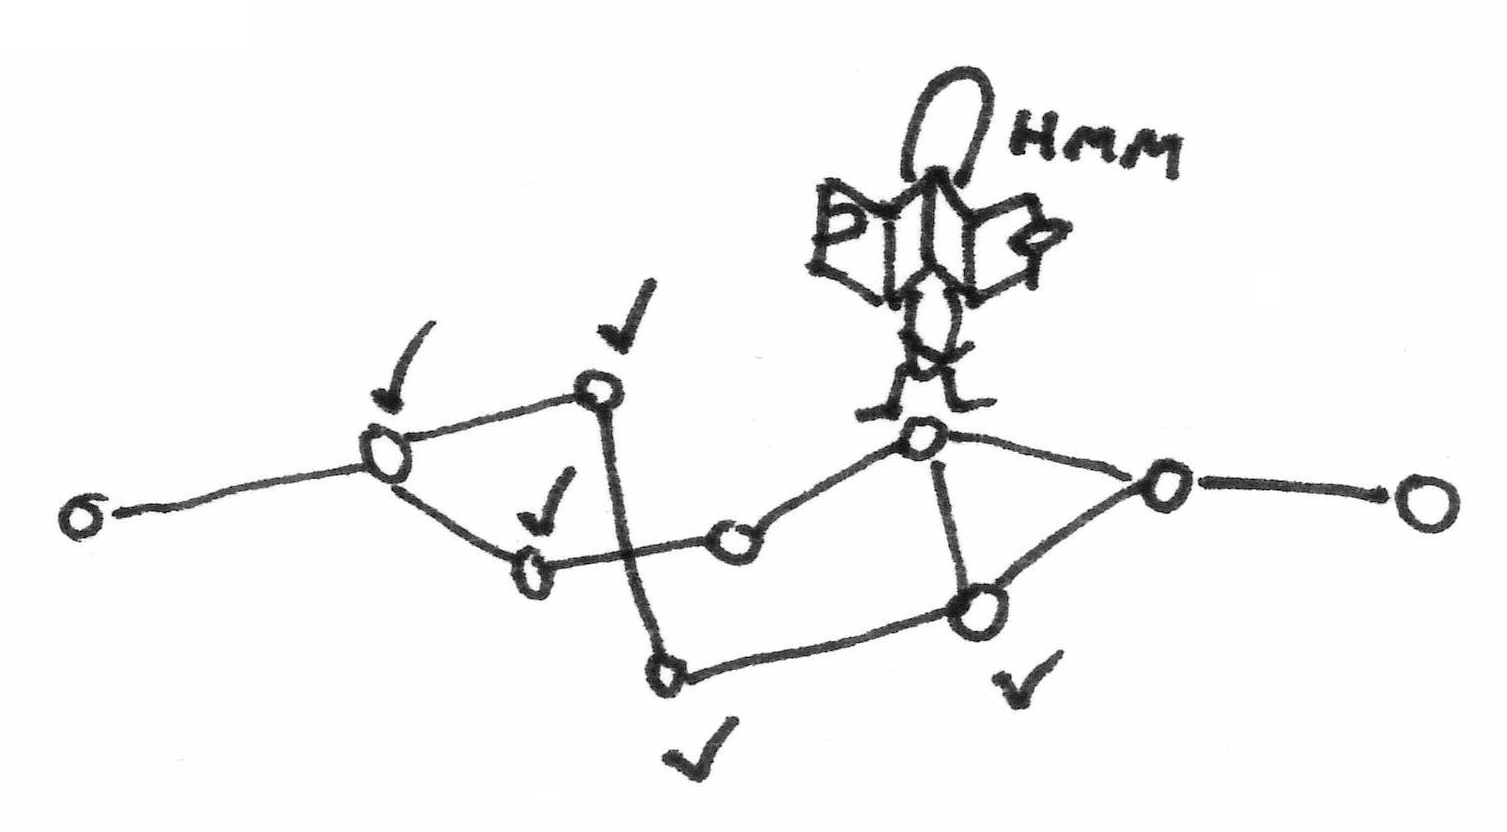
\includegraphics[scale=0.15]{../illustrations/graph-traversal}
\end{center}
\vspace{-1em}
\end{wrapfigure}
\fi

This is a challenge problem for deterministic-by-construction parallel
programming models. Existing parallel solutions (such as, for instance, the
parallel breadth-first graph traversal implementation from the
Parallel Boost Graph Library~\shortcite{bfs-pbgl}) often traverse the
connected component in a nondeterministic order---even though the
outcome of the program, that is, the final connected component, is
deterministic.  Neither IVars nor streams provide a way 
to orchestrate this traversal.  For
example, IVars cannot accumulate sets of visited nodes, nor can they
be used as ``mark bits'' on visited nodes, since they can only be
written once and not tested for emptiness.  Streams, on the other
hand, impose an excessively strict ordering for computing the
unordered \emph{set} of vertex labels in a connected component.
Before turning to an LVar-based approach, though, let us consider
whether a purely functional (and therefore deterministic by
construction) program can meet the specification.

\subsection{A purely functional attempt}

\singlespacing \lstinputlisting[float, caption={A purely functional
    Haskell program that finds the connected component of the
    \lstinline|profiles| graph that is reachable from the node
    \lstinline|profile0|, then maps the \lstinline|analyze| function
    over the nodes found.  Although component discovery proceeds in
    parallel, we cannot call \lstinline|analyze| on any of the nodes
    in the connected component until they have all been discovered.},
  label=listing-bfs_pure]{chapter2/code/bfs_pure.hs} \doublespacing

Listing~\ref{listing-bfs_pure} gives a Haskell implementation of a
\emph{level-synchronized} breadth-first graph traversal that finds the
connected component reachable from a starting vertex.  Nodes at
distance one from the starting vertex are discovered---and set-unioned
into the connected component---before nodes of distance two are
considered.  Level-synchronization necessarily sacrifices some
parallelism: parallel tasks cannot continue discovering nodes in the
component before synchronizing with all other tasks at a given
distance from the start.  Nevertheless, level-synchronization is a
popular strategy for implementing parallel breadth-first graph
traversal.  (In fact, the aforementioned implementation from the
Parallel Boost Graph Library~\shortcite{bfs-pbgl} uses
level-synchronization.)

Unfortunately, the code given in Listing~\ref{listing-bfs_pure} does
not quite implement the problem specification given above.  Even
though connected-component discovery is parallel, members of the
output set do not become available to @analyze@ until component
discovery is \emph{finished}, limiting parallelism: the first nodes in
the connected component to be discovered must go un-@analyze@d until
all of the nodes in the connected component have been traversed.  We
could manually push the @analyze@ invocation inside the @bf_traverse@
function, allowing the @analyze@ computation to start sooner, but
doing so just passes the problem to the downstream consumer, unless we
are able to perform a heroic whole-program fusion.

If @bf_traverse@ returned a list, lazy evaluation could make it
possible to \emph{stream} results to consumers incrementally.  But
since it instead returns a \emph{set}, such pipelining is not
generally possible: consuming the results early would create a proof
obligation that the determinism of the consumer does not depend on the
order in which results emerge from the producer.\footnote{As intuition
  for this idea, consider that purely functional set data structures,
  such as Haskell's \lstinline|Data.Set|, are typically represented
  with balanced trees.  Unlike with lists, the structure of the tree
  is not known until all elements are present.}

A compromise would be for @bf_traverse@ to return a list of
``level-sets'': distance one nodes, distance two nodes, and so on.
Thus level-one results could be consumed before level-two results are
ready.  Still, at the granularity of the individual level-sets, the
problem would remain: within each level-set, one would not be able to
launch all instances of @analyze@ and asynchronously use those results
that finished first.  Moreover, we would still have to contend with
the problem of separating the scheduling of producers and consumers
that pure programming with futures presents~\cite{monad-par}.

\subsection{An LVar-based solution}

Consider a version of @bf_traverse@ written using a programming model
with limited effects that allows \emph{any} data structure to be
shared among tasks, including sets and graphs, so long as that data
structure grows monotonically.  Consumers of the data structure may
execute as soon as data is available, enabling pipelining, but may
only observe irrevocable, monotonic properties of it. This is possible
with a programming model based on LVars.  In the rest of this \either{chapter}{section},
\either{I}{we} will formally introduce LVars and the $\lambdaLVar$ language and
give a proof of determinism for $\lambdaLVar$.  Then, in
\either{Chapter}{Section}~\ref{ch:quasi}, \either{I}{we} will extend the basic LVars model with
additional features that make it easier to implement parallel graph
traversal algorithms and other fixpoint computations, and \either{I}{we} will
return to @bf_traverse@ and show how to implement a version of it
using LVars that makes pipelining possible and truly satisfies the
above specification.
